\documentclass[12pt, a4paper]{article}
\usepackage{fontenc}
\usepackage{graphicx}
\usepackage{amsmath}
\graphicspath{ {./images/} }
\usepackage[ddmmyyyy]{datetime}
\usepackage{pdflscape}
\usepackage{subcaption}
\usepackage{url}
\renewcommand{\dateseparator}{.}
\renewcommand{\contentsname}{İçindekiler}
\renewcommand{\figurename}{Şekil}
\renewcommand{\refname}{Kaynakça}
\renewcommand{\tablename}{Tablo}
\usepackage{amsmath}
\usepackage{xcolor}
\title{\textbf{Videodan Animasyon Oluşturulması}\large }
\author{\textbf{İlknur Koparır}\large}
\date{\textbf{\today}}

\makeatletter         
\def\@maketitle{
\textbf{\large{T.C KÜTAHYA SAĞLIK BİLİMLERİ ÜNİVERSİTESİ}}\\[4ex]
\textbf{\large{MÜHENDİSLİK VE DOĞA BİLİMLERİ FAKÜLTESİ}}\\[4ex]

	\centering
	
\includegraphics[width = 60mm]{muh_logo.png}\\[8ex]
	\begin{center}
		{\large \bfseries \@title }\\[2ex] %\Huge
		{\small  \@author}\\[4ex] 
		
		\vspace{3\baselineskip}
		{\large \bfseries \subitem}
		\section*{\centering Danışman}
		\section*{\small \centering Dr.Öğr.Üyesi Emre Güngör}
		\section*{\small Yapay Zeka \& Veri Odaklı Sistem Tasarımı \& Latex İle Rapor Hazırlama}
		\vspace{2\baselineskip}
		\@date 
\end{center}}
\makeatother


\begin{document}
	
	\maketitle
	
	\thispagestyle{empty}
	
	\newpage

	\pagenumbering{arabic}
	\newpage

\newpage
\section{Giriş}  Hareket yakalama teknolojisi (motion capture), yüzyılı aşkın bir süre içerisinde
insanlığın geliştirdiği teknolojinin etkileri ile büyük ölçüde gelişim göstermiştir.
Günümüzde sanat, eğlence ve teknoloji dünyasında önemli bir yere sahip olan motion capture,insanların gerçek dünyadaki hareketleri dijital ortama aktarma ihtiyacından doğmuştur.Özellikle sinema, video oyunları,
reklam endüstrisi gibi alanlarda, gerçekçi hareketlerin oluşturulması ve karakterlerin doğal bir şekilde davranması büyük bir talep görmesinden dolayı bu teknolojilerin kullanım alanları gelişmektedir.Hareket halindeki bir obje veya bir canlının üç boyutlu koordinat ve açısal değişimlerinin çeşitli yöntemlerle
bir alıcıya iletilmesi olarak tanımlanan hareket yakalama teknolojisi  \cite{ozkiricscci2022motion}, işaretleyici tabanlı ve işaretleyici tabanlı olmayan sistemler
olarak ikiye ayrılmıştır. İşaret tabanlı hareket yakalama sistemleri manyetik veya optik vericilerin insan vücudunun önemli eklem bölgelerine yerleştirilerek hareket bilgisinin üretilmesidir. İşaret tabanlı olmayan hareket tanıma sistemlerde ise verici doğrudan figür olarak karşımıza çıkmaktadır.Kameralar, insan formunu arka plandan ayrıt eden algoritmalar ve derin öğrenme teknikleri sayesinde verilerden hareket bilgisi çıkarılmaktadır.Bu teknolojiler sayesinde  daha hızlı ve hassas hareket yakalama sistemleri geliştirilerek, gerçek zamanlı etkileşimli uygulamaların performansı artırılmakta ve kullanıcı deneyimi iyileştirilmektedir.\\
\begin{figure}[h!]
	\centering
	\begin{subfigure}[b]{0.4\linewidth}
		\includegraphics[width=5 cm, height=5 cm]{işaretTabanli.png}
		\caption{}
	\end{subfigure}
	\begin{subfigure}[b]{0.4\linewidth}
		\includegraphics[width=5 cm , height=5 cm]{işaretTabanliOlmayan.png}
		\caption{}
	\end{subfigure}
	\caption{(a) Manyetik hareket yakalama sistemi, (b) İşaretleyici tabanlı olmayan hareket yakalama sistemi.}
\end{figure}
\newpage
\section{Literatür Taraması}

Motion capture teknolojisinin kökenleri, eski çağlardan başlayarak, insanların hareketlerini taklit etme ve canlandırma ihtiyacıyla başlamıştır.

1906’da Amerikalı mucit Thomas Edison’un yardımı ile Amerikan gazetesi karikatüristi
James Stuart Blacton’un, Şekil \ref{fig:boat1}'de görüldüğü üzere ilk çizgi filmi olan Humorous Phases Faces’i (Komik Yüzlerin Mizahi
Evreleri) gösterime girmiştir.Çizgi filmde, kara tahta üzerinde, bir şapka ile oynayan palyaço ve çemberden atlayan bir köpek de dahil olmak üzere, elle çizilmiş karakterler bulunmaktaydı. Hareket ettirip durdurma tekniği kullanılan filmde, çizimler kendi başlarına tamamlanıyor ve sonra hareket eden çizimler gibi görünmekteydi. Bu teknik izleyiciler tarafından komik bulunmuş ve ilgi ile karşılanmıştır \cite{erdem2021sanali}

\begin{figure}[!h]
	\centering
	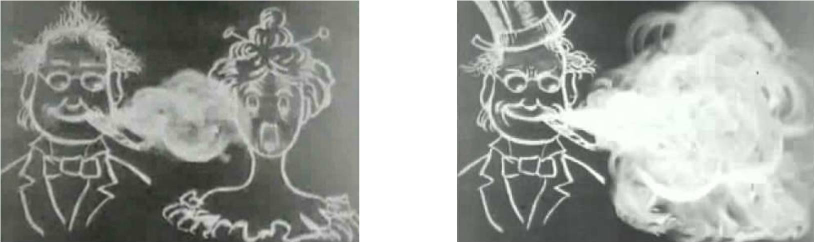
\includegraphics[width=10 cm , height = 3 cm ]{film.png}
	\caption{Humorous Phases Faces}
	\label{fig:boat1}
\end{figure}


1959’da Harrison, potansiyometrelerle (ayarlanabilir
dirençler) donatılmış bir elbiseyi oyuncuya giydirmiş ve oyuncunun tüm hareketlerini bir ekran
yardımı ile gerçek zamanlı olarak kaydetmeyi başarmıştır. Bu ilkel bir teçhizattı ancak gerçek
zamanlı hareket yakalamanın ilk örneğidir. 1980’lere gelindiğinde animatörler,
oyuncuların hareketlerini izlemek için aktif işaretçilerle kaplı vücut giysileri ve avuç
büyüklüğünde kameralar kullanmışlardır \cite{erdem2021sanali}. \\

Teknolojinin gelişmesiyle birlikte Rosales ve ark. \cite{rosalesestimating}, kalibre edilmemiş birden fazla görüş kullanılarak 3B eklemli duruşun (pose) tahmini için bir çerçeve sunar. Bu çerçevede, Uzmanlaştırılmış Haritalama Mimarisi (SMA) adı verilen istatistiksel bir çıkarım yöntemi kullanılır. SMA, kareler ve görünümler arasında 2B eklem konumları sağlar.\\

Kakadiaris ve Metaxas \cite{desmarais2021review} , dik açılı konfigürasyonlarda çoklu kamera görüntülerini kullanarak insan vücut parçalarının 3B model tabanlı izleme ve şekil tahmini için bir yöntem sunarlar. Daha sonra yaklaşımı, çoklu görüşlü video dizilerinden insan hareketinin tahmini ve buna göre animasyon dizileri oluşturmak için genişlettiler . 

\newpage
\section{Yöntem}
İnsan vücut hareketlerini kaydetmek ve dijital ortama aktarmak, günümüzde animasyon endüstrisinde ve interaktif teknolojilerde önemli bir rol oynamaktadır.
\subsection{Mediapipe}
Mediapipe, Google tarafından geliştirilmiş ücretsiz ve açık kaynaklı bir makine öğrenmesi kütüphanesidir.\cite{benefits}  Medya akışı (video, ses) üzerinde gerçek zamanlı veri işleme, nesne tespiti, nesne takibi, el ve yüz algılama gibi çeşitli görevleri gerçekleştirmek için tasarlanmıştır.\cite{chatgpt} MediaPipe'ın Holistic yöntemi, aynı anda yüz, el ve vücut pozisyonlarının  takibini mümkün kılmaktadır.Bu yöntem, Şekil \ref{fig:mesh1}'de görülebileceği üzere tek bir kare üzerinden 33 noktanın tespit edilmesine izin verirken, geleneksel COCO topolojisinde tek bir kare üzerinde 17 noktanın tespit edilmesini mümkün kılmaktadır.Bu yöntemle, 33 poz, 21 el ve 468 yüz işaret noktası olmak üzere toplamda 543 işaret noktası tespit edilebilir.Proje kapsamında OpenCV ve MediaPipe kütüphaneleri birlikte kullanılarak kamera üzerinde insan vücudunun tespiti yapılmıştır. Bu yöntemle, kameradan alınan görüntüler gerçek zamanlı olarak işlenerek insan vücudunun çeşitli parçaları, yani yüz, el ve vücut pozisyonları tespit edilmiştir. MediaPipe ile tespit edilen vücut parçalarının x, y, z koordinatları daha sonra kullanılmak üzere kaydedilmiştir.

\begin{figure}[h]
	\centering
	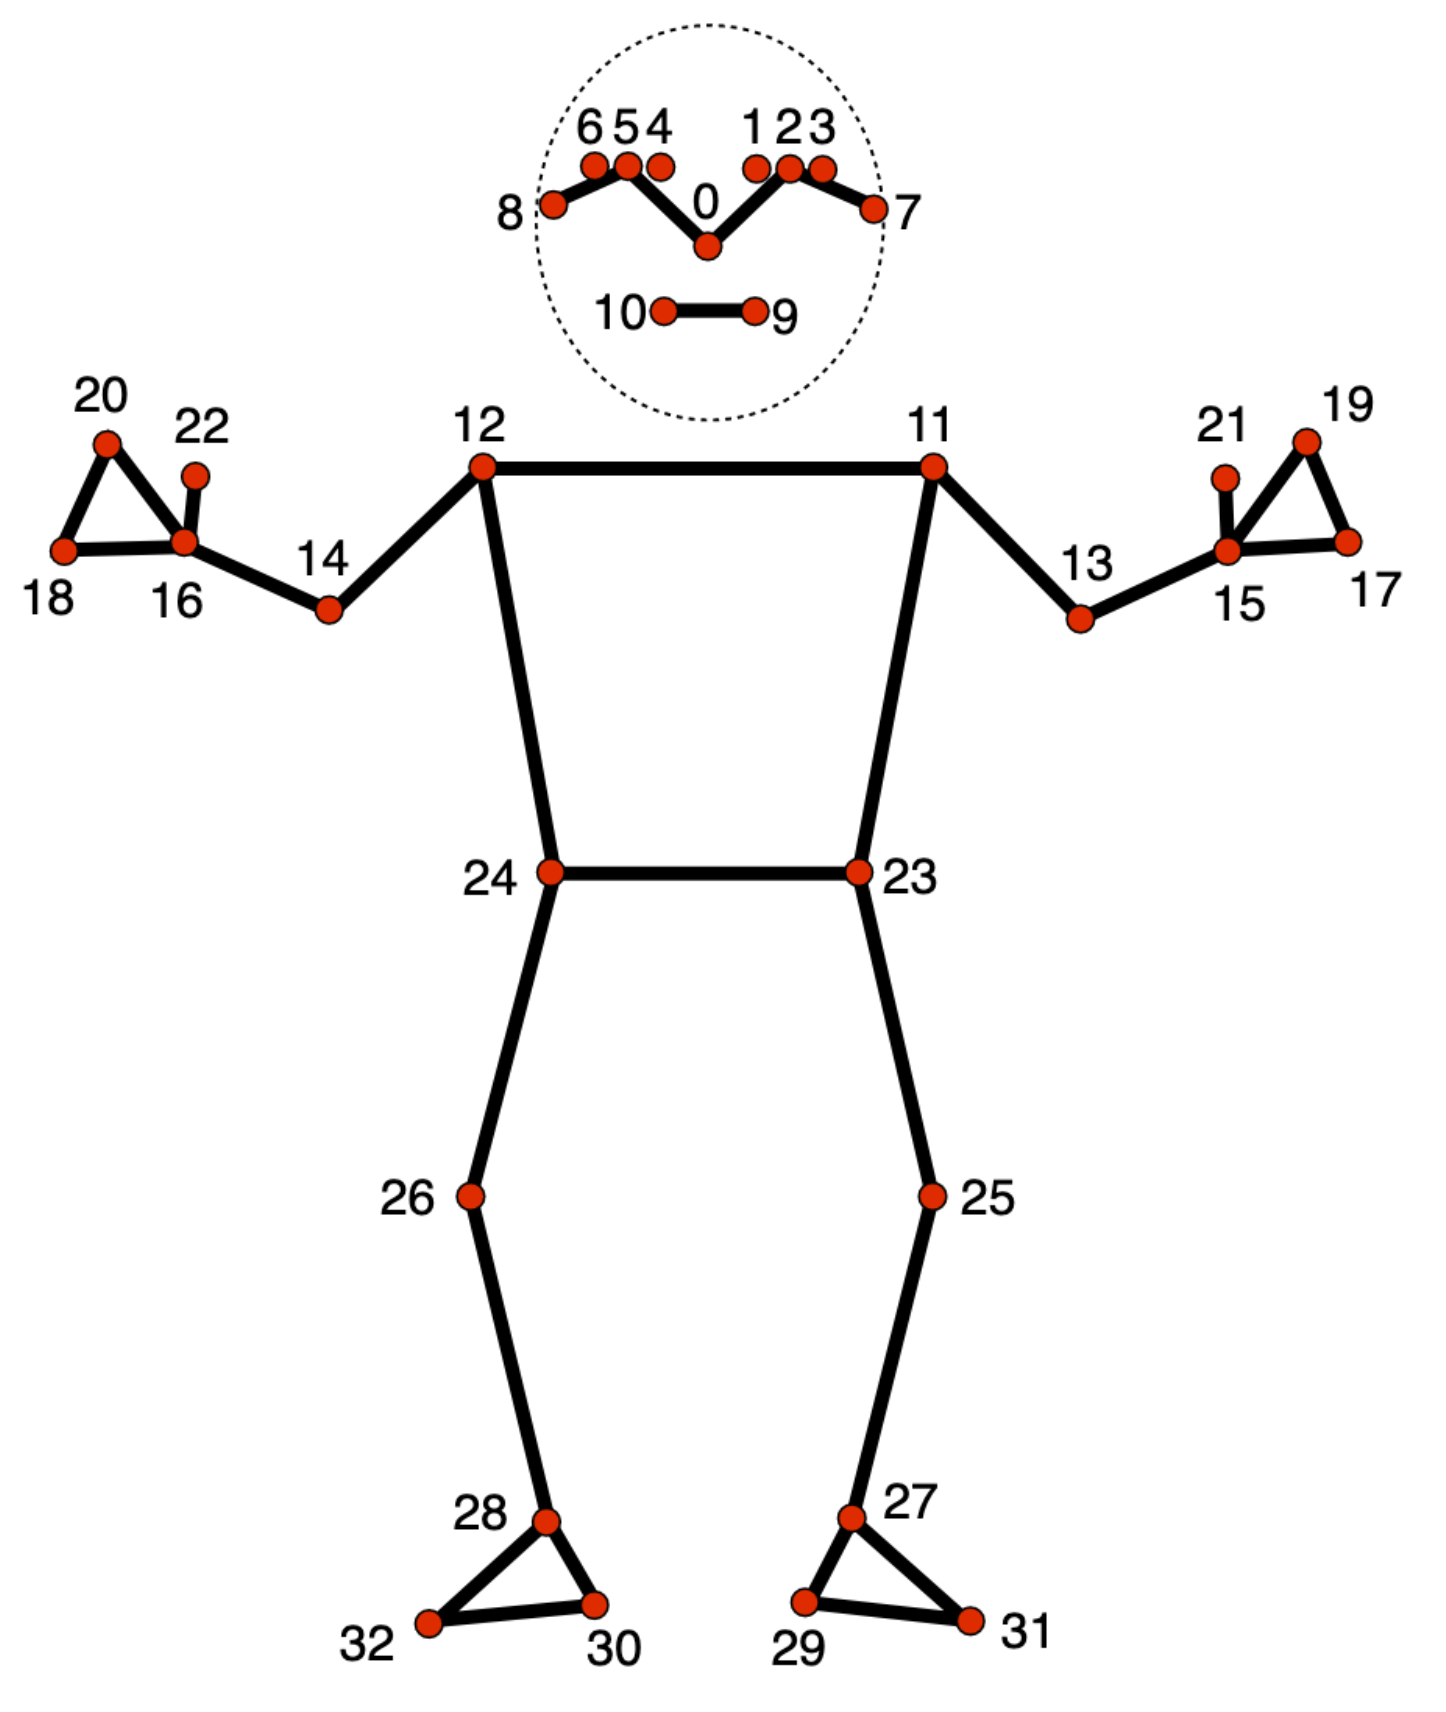
\includegraphics[width= 8 cm , height= 6 cm]{pose_landmarks_index.png}
	\caption{MediaPipe'da 33 vücut parçasının konumu \cite{benefits}}
	\label{fig:mesh1}
\end{figure}

\subsection{Blender ve Mixamo}

Mixamo, Adobe tarafından sunulan bir hizmet olup, sanat projelerinde, filmlerde ve oyunlarda kullanılmak üzere herkesin erişebileceği çevrim içi bir karakter ve mocap animasyon veritabanıdır.\cite{mixamo} Blender ise açık kaynak kodlu bir üç boyutlu modelleme ve animasyon yazılımıdır.Blender ile animasyon, görsel efekt, üç boyutlu model ve sanal gerçeklik modelleri üretiminde kullanılmaktadır.\cite{blender} 
\newline
\subsection{3D Karakter Modeli}
Animasyon projeleri için özel karakter modeli bulunmuyorsa Mixamo kullanmamız için  önceden  hazırlanmış karakterler sunmaktadır. Karakterler projede kullanılmak üzere .fbx formatında indirilmesi gerekmektedir.
\begin{figure}[h]
	\centering
	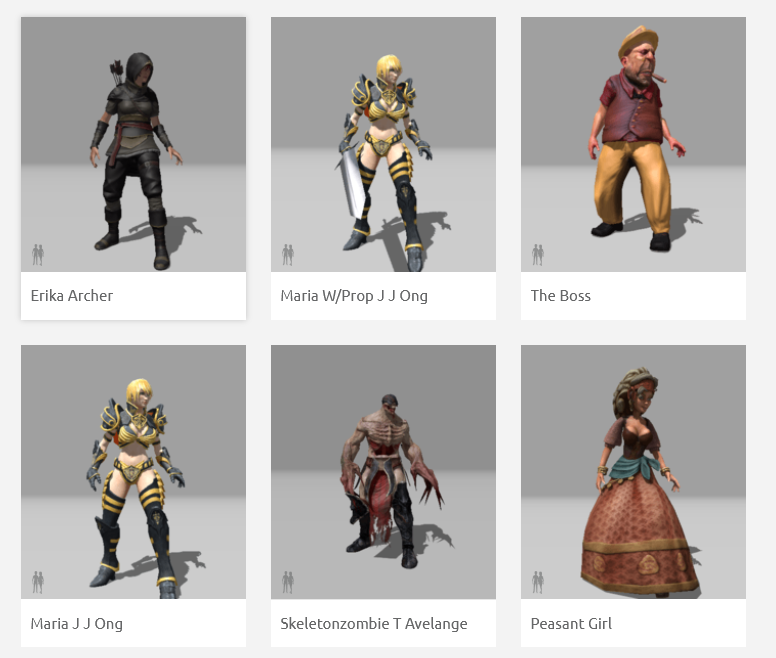
\includegraphics[width= 15 cm, height = 10 cm]{karakter.png}
	\caption{Mixamo da bululnan hazır karakterlerden bazıları} \cite{mixamo-2}
\end{figure}
\newpage
\subsection{Blender ortamında karaktere iskelet yerleştirilmesi}
Mixamo'dan indirilen karaktere hareket vermek için Blender üzerinden iskelet yerleştirme işlemi yapılmıştır. Bu işlem, karakterin hareket edebilmesi ve animasyonlarının uygulanabilmesi için gerekli temel yapıyı oluşturur. İskelet, karakterin vücut yapısına uygun olarak düzenlenerek  eklem bölgeleri doğru şekilde konumlandırılmıştır.

\begin{figure}[h]
	\centering
	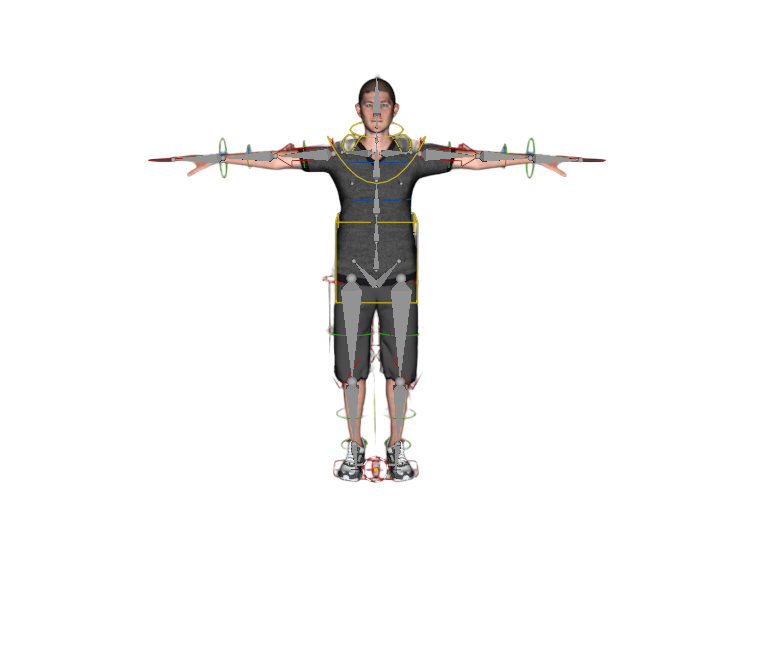
\includegraphics[width= 15 cm, height = 9 cm]{iskelet-Photoroom.png}
	\caption{Blender ortamında karaktere iskeletin yerleştirilmesi ve ağırlıklandırılmasının yapılması.}
	
\end{figure}

\subsection{Rokoko}
Rokoko Studio eklentisi, Blender'da animasyon oluşturmak için kullanılan bir araçtır.Bu eklenti sayesinde, hareket yakalama verileri dijital karaktere kolaylıkla aktarılabilmektedir.\cite{chatgpt}

\subsubsection{Blender Ortamında Karaktere Hareket Verilmesi}
Karaktere hareket verilmek üzere blender da Retargeting paneli açılmıştır.
Bu panel, animasyonların yeniden hedeflenmesi işlemlerini gerçekleştirmemize olanak sağlamaktadır. Ardından animasyonun kaynak iskeletini ve animasyonun hedef alınacağı iskelet seçilmiştir. Kaynak iskelet, animasyonun geldiği orjinal iskeleti temsil ederken, hedef iskelet, animasyonun yeniden hedefleneceği iskeleti temsil eder. Bu adımda, Blender'ın bu iki iskelet arasındaki kemik listesini oluşturması için "Build Bone List" işlemi yapılmıştır. Kemiklerin doğru eşleştirildiğinden emin olmak için Blender'ın oluşturduğu kemik listesini kontrol edilmiştir. Eğer eksik veya yanlış kemikler varsa, bunların düzeltmesi yapılır.Ardında animasyona hareket verilmiştir.
\begin{figure}[h]
	\centering
	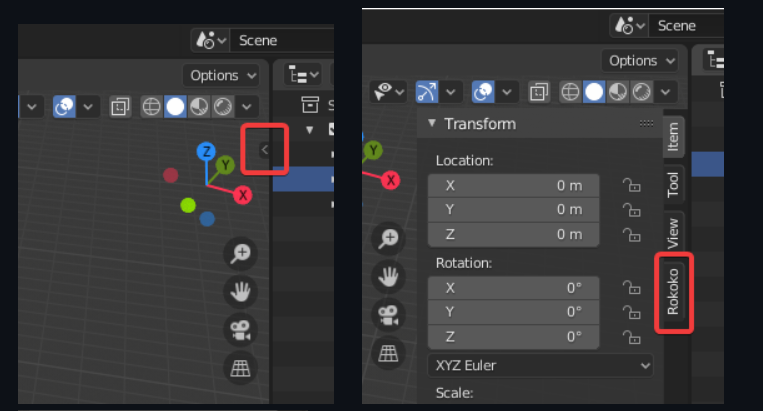
\includegraphics[width= 7 cm , height= 5 cm]{rokoko1.png}
	\caption{Retargeting.}
\end{figure}


\begin{figure}[h]
	\centering
	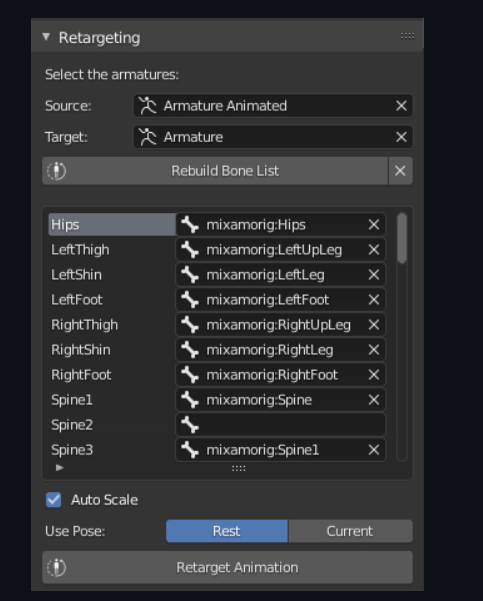
\includegraphics[width=6 cm , height= 7 cm]{rokoko4.png}
	\caption{İki iskelet arasında kemiklerin eşleştirilmesi.}
\end{figure}
\begin{figure}[h]
	\centering
	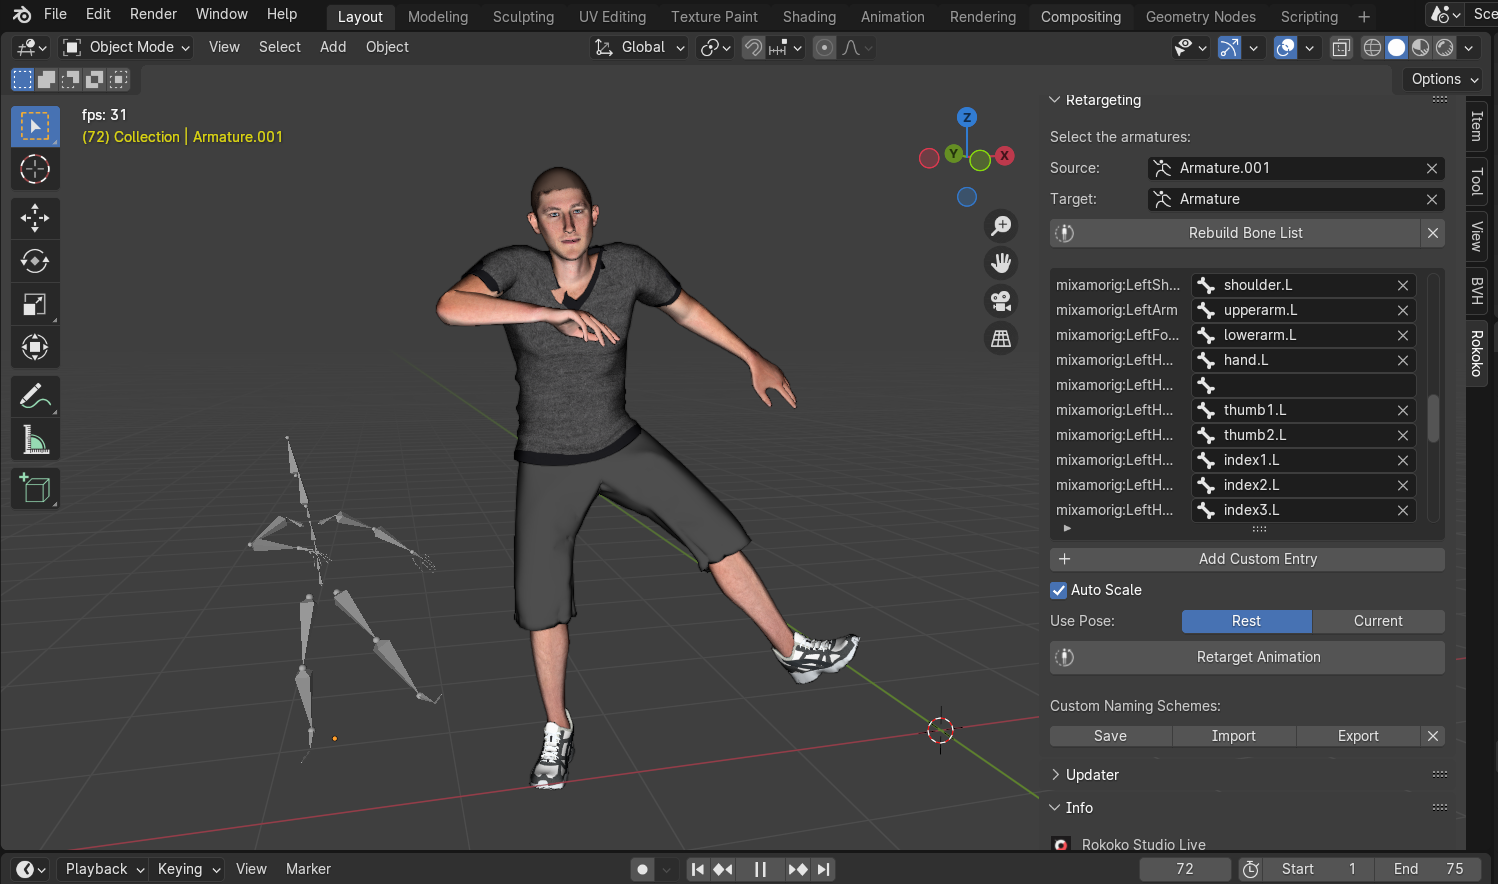
\includegraphics[width= 15 cm , height= 10 cm]{pose2.png}
	\caption{Retargeting.}
\end{figure}



\subsection{Bvh Dosya Formatı}
BVH dosya formatının geçmişi ve gelişimi 1990'lara kadar uzanır ve başlangıçta BioVision'ın hareket yakalama sistemleri için özel bir dosya formatı olarak geliştirilmiştir.BVH'den önce hareket verileri kalem ve kağıtla kaydediliyor ya da bilgisayara manuel olarak giriliyordu. BVH, hareket verilerinin otomatik olarak yakalanmasını ve kaydedilmesini sağlayarak gerçekçi animasyonlar oluşturmayı daha kolay ve verimli hale getirdi.

Günümüzde BVH, hareket yakalama verileri için yaygın olarak kullanılan bir dosya formatı olmaya devam etmektedir ve Autodesk'in Maya ve Blender gibi birçok animasyon yazılım paketi tarafından desteklenmektedir. Animasyon endüstrisinde, özellikle filmler ve video oyunları için gerçekçi ve gerçeğe yakın animasyonlar oluşturmak için önemli bir araç haline gelmiştir.\cite{biovision-file-format-1}
\begin{figure}[h]
	\centering
	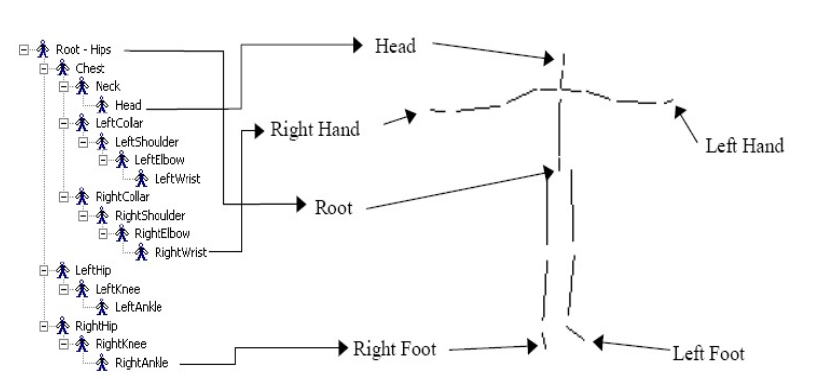
\includegraphics[width=8.5 cm , height = 5 cm ]{bvhyeni.png}
	\caption{BVH iskelet yapısı} \cite{biovision-file-format-2}
\end{figure}
\subsection{BVH Formatı Terminoloji}
Hareketi tanımlamak için kullanılan anahtar kelimelerden bazıları aşığıda özetlenmiştir.
\begin{itemize}
	\item{\textbf {İskelet}}: Hareketin temsil ettiği karakterin tamamı.
	\item {\textbf {Kemik}}: Hareket içindeki en küçük parça.İskeletler bir dizi kemikten oluşur.
	\item {\textbf {Kanal veya özgürlük derecesi (DOF)}}: Bir kemiğin animasyon sırasında değiştirebileceği parametredir. Bir kemik, konum, yön ve ölçek olmak üzere üç ana eksende hareket edebilir. Her eksen, bir DOF olarak kabul edilir..
	\item {\textbf {Çerçeve}}: Çerçeve, bir animasyondaki belirli bir zaman noktasını temsil eder. Her çerçeve, animasyondaki her bir kemiğin o zamandaki konumunu, yönünü ve ölçeğini tanımlar..
	
\end{itemize}

\subsection{BVH Formatı Çalışma Prensibi}
Dosyanın hiyerarşik bölümü HİYERARŞİ anahtar kelimesi ile başlar ve bunu bir sonraki satırda ROOT
anahtar kelimesi ve iskelet hiyerarşisinin kökü olan kemiğin adı takip eder. ROOT anahtar sözcüğü, yeni
bir iskelet hiyerarşik yapısının başlangıcını belirtir ve BVH dosyası birçok iskelet içerme kapasitesine
sahip olmasına rağmen, genellikle dosya başına yalnızca tek bir iskeletin tanımlanması gerekir.İskeletin geri kalan yapısı yinelemeli bir yapıda tanımlanır.Her bir düğümün, OFFSET, CHANNELS ve JOINT gibi özellikleri vardır. OFFSET, Her eklemin, ebeveyn ekleme göre yer değiştirmesini belirtir.. CHANNELS, düğümün dönme bilgilerini temsil eder. JOINT, düğümün bir eklem noktasını temsil ettiğini belirtir ve altında başka düğümler bulunabilir.Endvsite ise Bir eklemin sonunu belirtir.\cite{article}


\section{Eksik Verilerin Tamamlanması}
Mediapipe ve Blender, karakter iskeleti tespiti ve animasyon oluşturma konularında farklı araçlar olsa da, bu iki platform arasında uyumluluk sağlamak oldukça önemlidir.
Mediapipe kütüphanesi, insan vücudunun iskeletini tespit ederken bazı kemikleri eksik bırakmaktadır.
Bu nedenle, eksik kemikleri tamamlayarak bunların x, y, z koordinatlarını bulmamız gerekmektedir.
Eksik olan boyun kemiğini tespit etmek için sol dudak ve sağ dudak orta noktasını tespit edip ardında sağ omuz ve sol omuzun orta noktası tespit edilir.Ardından tespit edilen bu iki noktanın da orta noktası tespit edilip bu noktaya boyun kemiği olarak işaretlenir.
\newline 

\begin{center}
	Orta noktanın x koordinatı: \( \frac{{x_1 + x_2}}{2} \) \\ 
	Orta noktanın y koordinatı: \( \frac{{y_1 + y_2}}{2} \) \\ 
	Orta noktanın z koordinatı: \( \frac{{z_1 + z_2}}{2} \)
\end{center}
\begin{figure}[h]
	\centering
	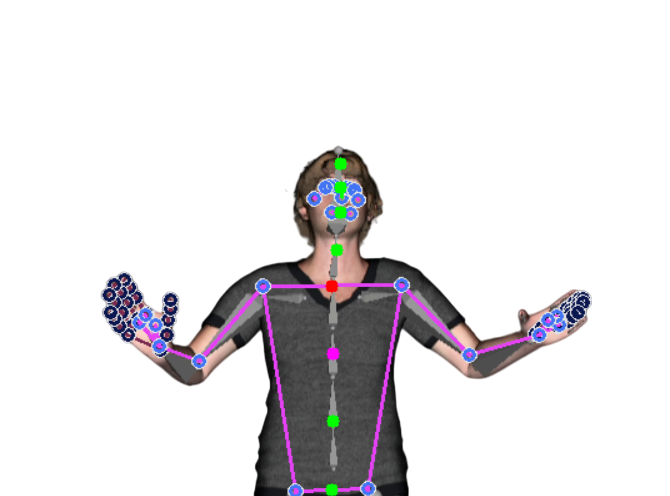
\includegraphics[width= 15 cm, height = 5 cm]{kemik-tamamlama.png}
	\caption{Eksik verilerin tamamlanıp kordinatlarının işaretlenmesi} 
\end{figure}

\begin{figure}[h] 
	\centering
	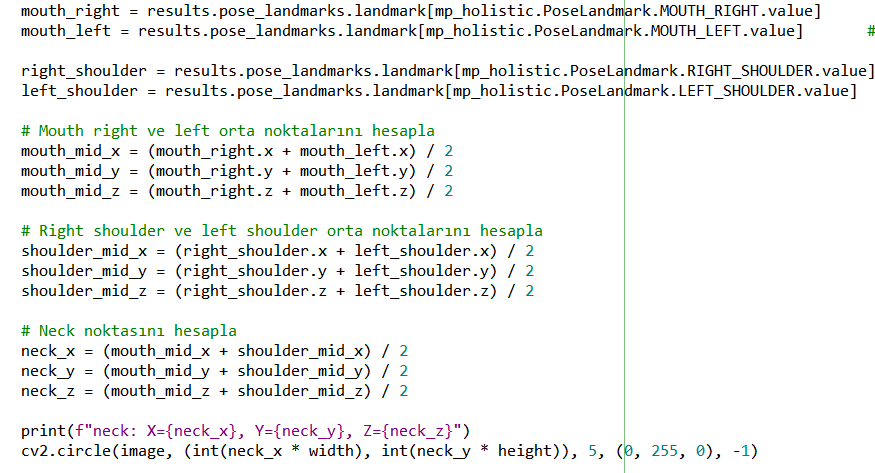
\includegraphics[width=15 cm , height = 7 cm ]{code1.png}
	\caption{Python da boyun kemiğinin konumunun hesaplanması.}
\end{figure}
Mediapipe kütüphanesi omurga kemiklerini tespit etmemektedir.Omurga kemiklerini hesaplamak için sol omuz ve sağ omuzun kemiklerinin orta noktası alındıktan sonra sol kalça ve sağ kalçanında orta noktası tespit edilir.Ardından tespit edilen bu iki nokta arasındaki mesafe 3 eşit noktaya ayırma işlemi yapılır.Tespit edilen noktalar opencv kütüphanesi ile işaretlenmiştir.
\begin{figure}[h!]
	\caption{Python da omurga kemiklerinin konumunun hesaplanması.}
	\centering
	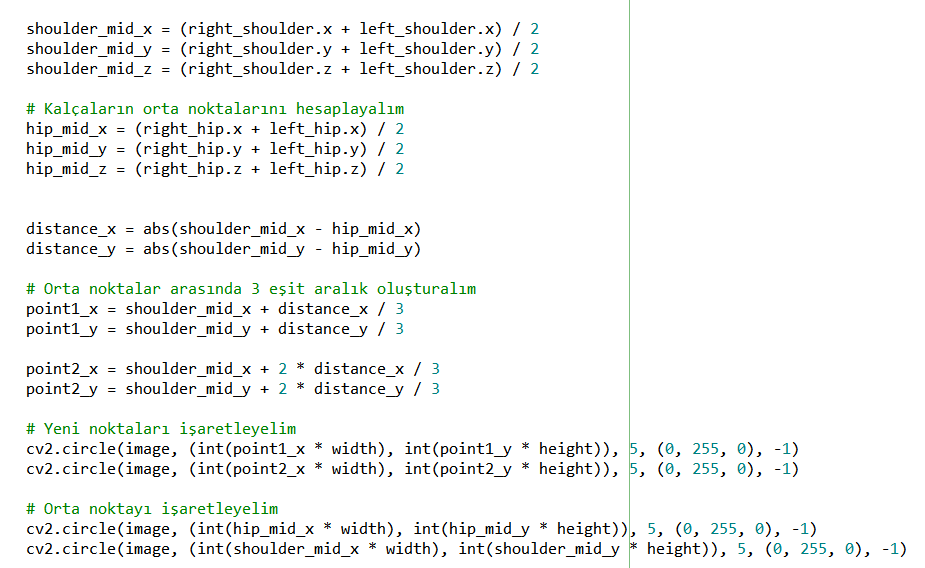
\includegraphics[width=18 cm , height = 8 cm]{code2.png}
\end{figure}
\subsection{ANTROPOMETRİK ÖLÇÜMLER}
Antropometri, Yunanca antropos (insan) ve metrein (belirleme, ölçü) sözcüklerinden oluşan ve insan vücudunun ölçülerini konu edinen bir bilim dalıdır.Bireyler veya gruplar arasında, anatomi, coğrafi bölge ve meslek grupları gibi çeşitli faktörlerden kaynaklanan farklılıkları ve benzerlikleri saptayarak daha geniş bir insan kitlesine uygun tasarımlar yapma imkânı sağlar.
\begin{figure}[h] 
	\centering
	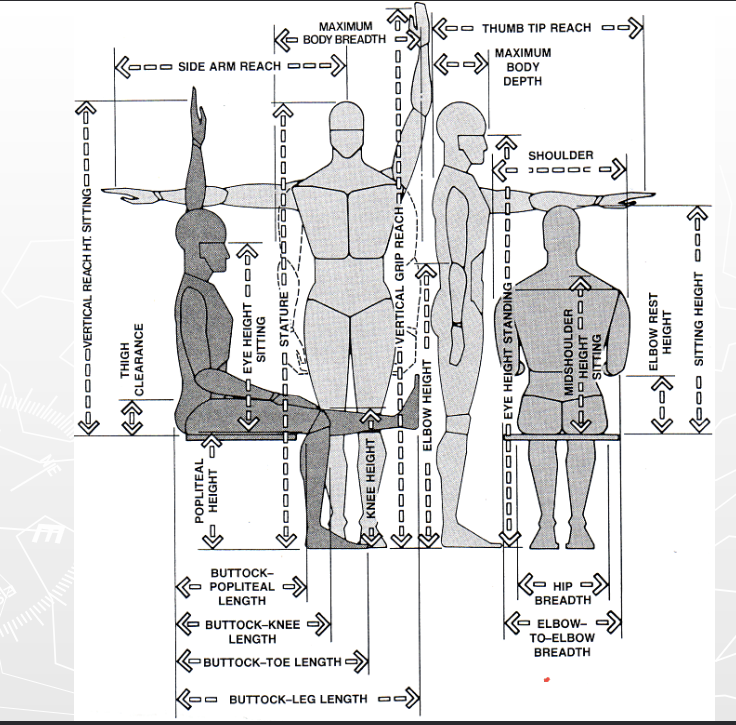
\includegraphics[width=8 cm , height = 7 cm ]{ant.png}
	\caption{Ölçüm noktaları.}
\end{figure}
\subsubsection{Baş Bölgesindeki Antropometrik Noktalar}
Başın konumu Oksipital çıkıntı ve kaşların üzerinden ölçülür.
\begin{figure}[h] 
	\centering
	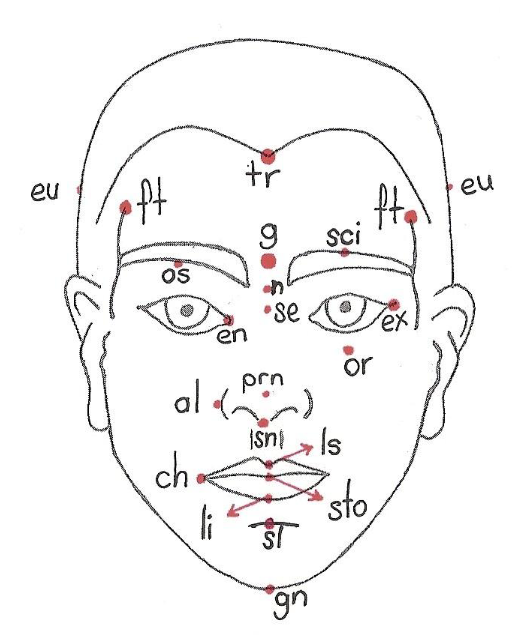
\includegraphics[width=8 cm , height = 5 cm ]{bas.png}
	\caption{ Önden görünüşte baş üzerindeki antropometrik noktalar.}
\end{figure}
\pagebreak

\begin{figure}[h!]
	\centering
	\begin{subfigure}[b]{0.4\linewidth}
		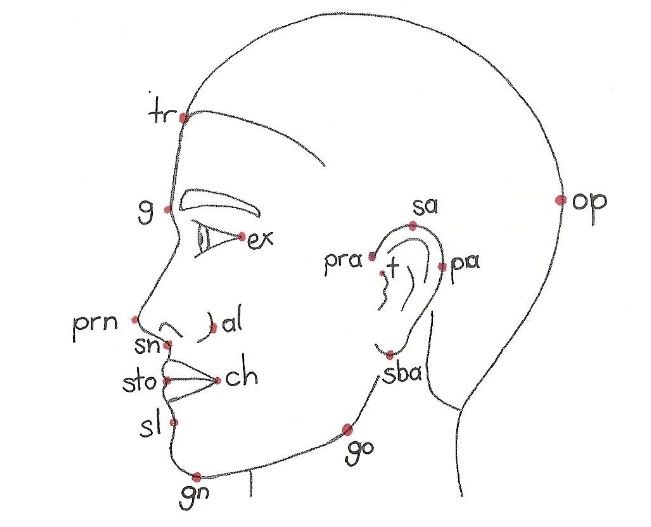
\includegraphics[width=5 cm, height=5 cm]{yan.png}
		\caption{}
	\end{subfigure}
	\begin{subfigure}[b]{0.4\linewidth}
		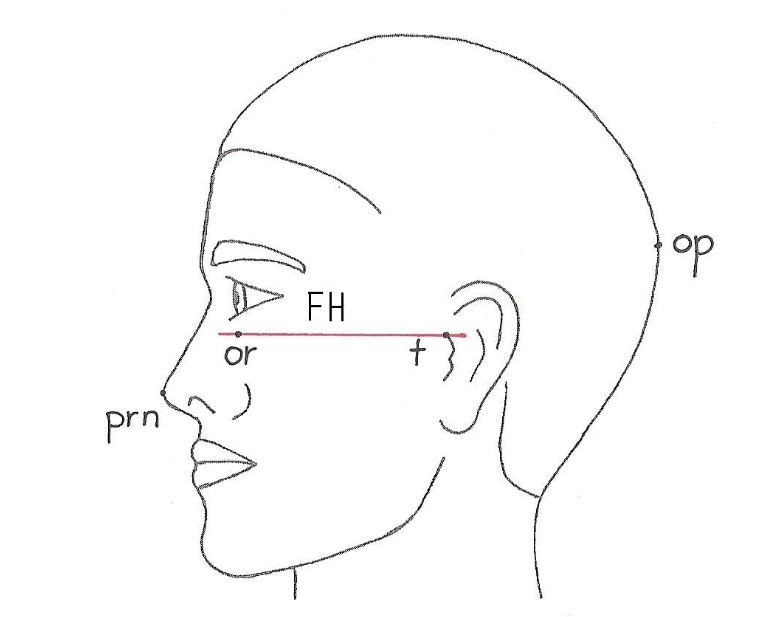
\includegraphics[width=5 cm , height=5 cm]{fh.png}
		\caption{}
	\end{subfigure}
	\caption{ (a) Yandan görünüşte, baş üzerindeki antropometrik noktalar. (b)  Başın standart pozisyonu FH}
\end{figure}

\subsection{Altın Oran}
Temelde, bir nesnenin veya bir yapıtın estetik olarak hoş ve dengeli görünmesini sağlamak için kullanılan bir oranı ifade eder. Eski Mısırlılar ve Yunanlılar
tarafından keşfedilmiş, mimaride ve sanatta kullanılmıştır.Sanatçılar, bilim adamları ve tasarımcılar,araştırmalarını yaparken ya da ürünlerini ortaya
koyarlarken orantıları altın orana göre belirlenmiş insan bedenini ölçü olarak alırlar.
Altın oran Deniz kabuğunun spiralinde, insan elinde, DNA diziliminde, Akciğerlerde ve uzayda olmak üzere pek çok yerde karşımıza çıkmaktadır.\newline

\fbox{
	\begin{minipage}{0.25\textwidth}
		\centering
		$\phi = \frac{1 + \sqrt{5}}{2}$
	\end{minipage}
}
\subsubsection{Yüzdeki Altın Oran}
Yüzde estetik bir görünüm elde etmek amacıyla kullanılan  matematiksel bir orandır. Bu oran, yüzdeki farklı bölgeler arasındaki oranları belirleyerek yüz hatlarının dengesini ve simetrisini değerlendirir. Altın Oran, genellikle gözler, burun ve ağız gibi temel yüz özellikleri arasındaki ilişkiyi inceler.
\begin{itemize}
	\item Alın yüksekliği Yüz uzunluğunun  yüzde 33'üne eşit olmalıdır.
	\item Burun uzunluğ  Alın yüksekliğinin yüzde 50'sine veya burun kökü ile çene ucu arasındaki mesafenin 33'üne eşit olmalıdır.
\end{itemize}

\section{Rotasyon İşlemleri}
Mediapipe ve Blender gibi farklı platformlar, farklı koordinat sistemlerini kullanır.Bu sistemlerdeki koordinatlar farklı yönlere veya orijinlere sahiptir. Mediapipe'de genellikle kamera görüş açısına göre tanımlanan bir koordinat sistemi kullanılırken, Blender'da dünya uzayına göre bir koordinat sistemi kullanır. Bu nedenle, Mediapipe'den gelen koordinatlar doğrudan Blender koordinatlarına uygulanamaz. 
Mediapipe'den gelen koordinatları Blender koordinat sistemine dönüştürmek için dönüşüm matrisleri kullanıyoruz.
\begin{center}
	Dönüşüm Matrisi Uygulanmadan Önce \\
	\textcolor{blue}{x:} 0.52258945 \\
	\textcolor{blue}{y:} 0.2965024 \\
	\textcolor{blue}{z:} -0.23053758 \\
\end{center}

\vspace{0.1cm}

\begin{center}
	Dönüşüm Matrisi Uygulandıktan Sonra \\
	\textcolor{red}{x:} 0.52258945 \\
	\textcolor{red}{y:} -0.23053758 \\
	\textcolor{red}{z:} 0.2965024
\end{center}
Dönme matrisin amacı Öklid uzayında vektörlerin rotasyonunu gerçekleştirmektir. Genellikle uzayı belirli bir açı veya derece etrafında döndürmek için kullanılır.
İki veya üç boyutlu uzayda nesnelerin konumlarını değiştirmek, yönelimlerini değiştirmek ya da vektörün Kartezyen koordinatlarını yeni korinatlarla eşlemek istediğimizde dönme matrisleri kullanılır.
Dönme matrisleri, bilgisayar grafikleri, robotik, bilgisayar görüşü gibi alanlarda yaygın olarak kullanılır. Özellikle 3D grafiklerde nesnelerin dönme ve yönlendirme işlemlerinde sıkça karşımıza çıkarlar.\newline \newline
\textbf{2D dönme matrisi:}
\[
\begin{pmatrix}
	\cos(\theta) & -\sin(\theta) \\
	\sin(\theta) & \cos(\theta)
\end{pmatrix}
\]
\newline
\textbf{3D dönme matrisi:}
\[
\begin{pmatrix}
	\cos(\theta) & -\sin(\theta) & 0 \\
	\sin(\theta) & \cos(\theta) & 0 \\
	0 & 0 & 1
\end{pmatrix}
\]
\section{Euler Formülü}
Euler dönüşleri, bir nesnenin 3D uzayda dönüşünü ifade etmek için kullanılan bir yöntemdir. Bu yöntemde, bir nesnenin dönme hareketi, üç farklı eksen etrafında gerçekleşen açısal değişikliklerle tanımlanır. Euler dönüşleri, nesnenin dönüşünü ifade etmek için üç açı kullanır bunlar sırasıyla roll, pitch ve yaw açılardır.

\begin{itemize}
	\item Roll açısı x eksenindeki dönüşü temsil eder.
	\item Pitch açısı y eksenindeki dönüşü temsil eder.
	\item Yaw açısı z eksenindeki dönüşü temsil eder. 
\end{itemize}

\section{Gimbal Lock}
Gimbal lock (Gimbal kilidi), 3D uzayda nesnelerin dönüşlerini ifade etmek için kullanılan Euler açılarının bazı durumlarda ortaya çıkan istenmeyen bir durumdur.

Gimbal sistemi, bir nesnenin üç eksen etrafında dönmesine izin veren bir mekanizmadır. Her eksen bir gimbal olarak adlandırılır ve bu eksenler birbirine dik olarak yerleştirilir. Ancak, Euler açıları kullanılarak nesnenin rotasyonu ifade edilirken, bu gimballer bazen birbirine hizalanabilir. Bu durumda, iki veya daha fazla eksen aynı hizada olduğunda, sistemde gimbal lock oluşur.
Bu durumda, belirli bir dönüş yönü veya açısal hareket kaybolabilir veya kısıtlanabilir. Özellikle, iki gimbal birbirine hizalandığında, üçüncü bir eksen etrafındaki dönüşün doğru bir şekilde ifade edilemez.
\section {Quarternion}
Euler açıları objelerin rotasyonlarını çözme konusunda insanın aklına gelen en doğal yöntem olsa da en optimal yöntem değil. Örneğin “Gimbal Lock” denilen problem euler açılarını kullandığımızda ortaya çıkıyor. Eksenlerimizdeki rotasyonlar üst üste bindiğinde sistemimiz kilitleniyor ve rotasyonları gösterme gücümüz azalıyor.



Bu sorunun yaşanmaması için Quaternion’lar kullanılıyor. Quaternion’larda Euler açılarına ek olarak 4. bir değer var. Bu değer skaler bir değer. Ve bu 4. değer sayesinde çakışmalar önleniyor.Kuvaterniyonlar (quaternion'lar), üç boyutlu uzayda dönüşümleri temsil etmek için kullanılan matematiksel yapılar olup kompleks sayılar üzerine genişletilmiş bir sayılar sistemidir. William Rowan Hamilton tarafından 1843 yılında geliştirilmiştir.  Kuvaterniyonlar, vektörlerin döndürülmesi, uzay geometrisinde rotasyonların tanımlanması ve fiziksel simülasyonlarda kullanılırlar


\begin{figure}[h]
	\centering
	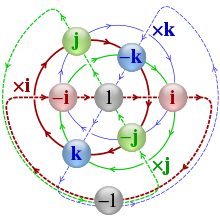
\includegraphics[width=8 cm  ,height=5 cm  ]{quaternion.png}
\end{figure}

\[
\boxed{q = a + bi + cj + dk}
\]
\begin{figure}[h]
	\centering
	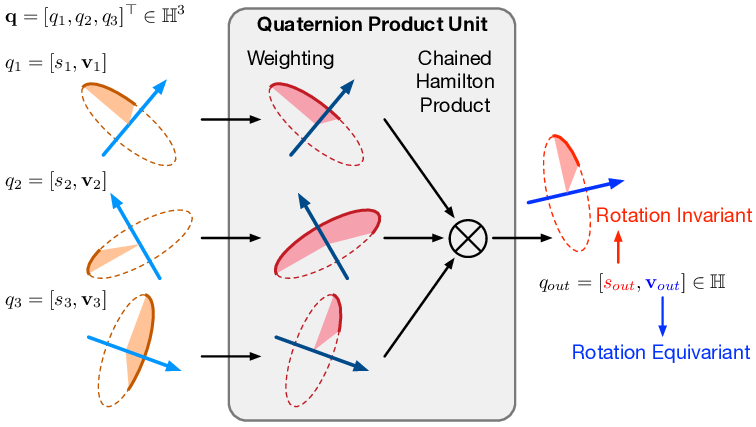
\includegraphics[width=10 cm  ,height=5 cm  ]{quaternion-1.png}
\end{figure}
\section{Unity ortamında iskelete hareket verilmesi}
 Vücut noktalarının x, y, z koordinatlarını kaydetmek ve bu verileri Unity ortamında kullanmak amaçlanmıştır. İlk olarak, 33 adet vücut noktasının koordinatlarını içeren bir animation.txt dosyası oluşturduk. Daha sonra, Unity ortamında her biri bir eklemi temsil eden 33 adet küre ekledik. Kaydettiğimiz animation.txt dosyasını, projedeki Asset klasörüne yapıştırarak Unity'de kullanılabilir hale getirdik. animation.txt dosyasındaki string formatındaki değerleri koordinatlara dönüştürmek amacıyla bir C# projesi oluşturduk. Her yerden erişilebilir bir Vücut adında game object oluşturduk ve bu game object'i yönetici bir script içine yerleştirdik. 33 adet landmark olduğu için Vücut nesnesinin değerini 33 yaparak, oluşturduğumuz kürelerle bu noktaları eşleştirdik.
\begin{figure}[h]
	\centering
	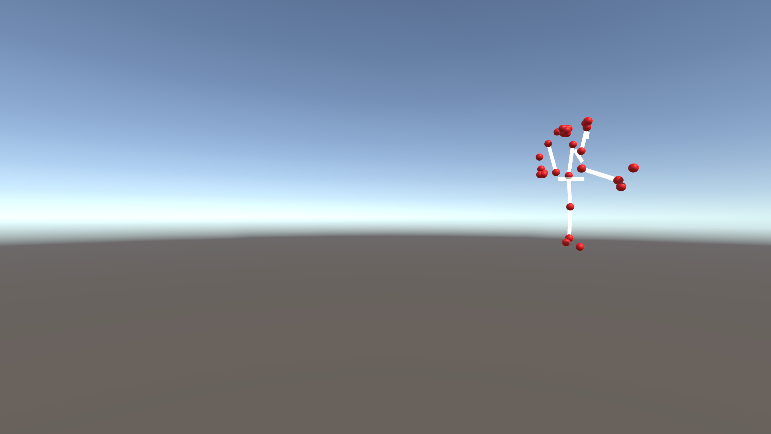
\includegraphics[width=8 cm , height = 7 cm ]{3-1.png}
	\caption{Unity ortamında motion capture.}
\end{figure}
 
\section{Alınan Hatalar}
Euler açısı kullanarak eklemlerin rotasyon hesaplaması yaparken çıkan sonuçlar hep 0 ve 1 arasında değerlerdir. Ancak hazır bvh dosyaları incelendiğinde eklemlerin rostasyon değerleri 0 ve 1 arasına sıkışmamış, çeşitli değerler almış.


 \begin{figure}[h]
	\centering
	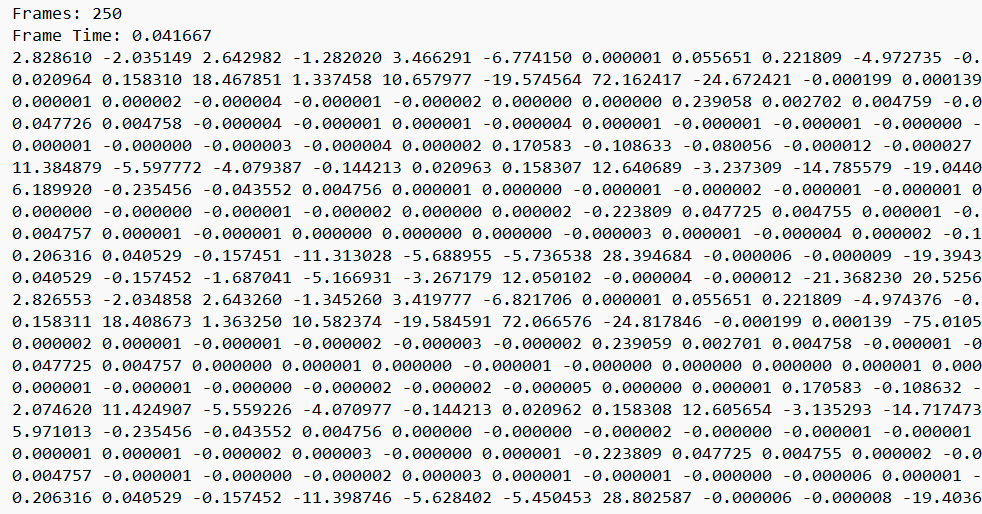
\includegraphics[width=12 cm , height = 7 cm ]{hata1.png}
	\caption{Olması gereken bvh formatı.}
\end{figure}

\begin{figure}[h]
	\centering
	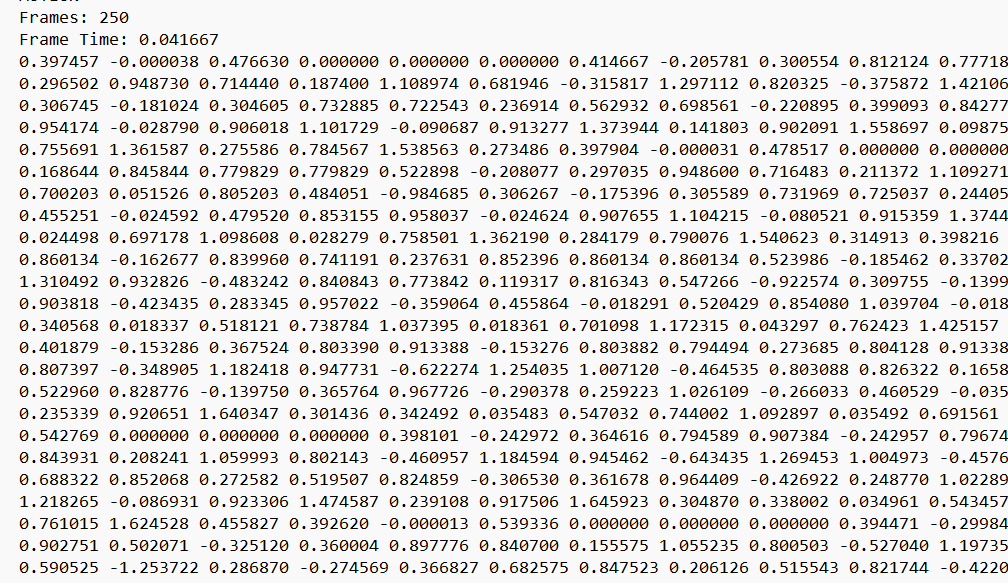
\includegraphics[width=12 cm , height = 6 cm ]{hata2.png}
	\caption{Euler açısı kullanarak elde ettiğim bvh dosyası.}
\end{figure}
\section{Bulgu ve Tartışma}
Vize öncesi hazırlanan gantt şemasında bvh dosya formatına 14 gün ayrılmıştır.Ancak projenin ilerleyen kısımlarında bizden eklemlerin x, y, z kordinatlarını değil x,y,z rotasyonlarını istediğini fark ettim. Bu yüzden kemiklerin euler açısı ile dönme kordinatlarını hesaplamaya çalıştım. Bu hesaplamaları yaparken birçok sorun ile karşılaştım ve dönme noktaları düzgünce hesaplanamadı. Bundan dolayı proje süresi uzamıştır. 
\section{Beklenen Sonuçlar}
Proje henüz tamamlanmadığı için beklenen sonuçlar yazılmıştır.
Hareket yakalama teknolojisi son yıllarda biyomekanik, yaya
navigasyonu, eğitim ve simülasyon, sanal gerçeklik ve
karakter animasyonu alanlarında oldukça önem kazanmıştır.
Bu çalışmada da hedeflenen sonuç kameradan alınan görüntü üzerinden vücut hareketlerini tespit edip bu hareketler 3 boyutlu olarak aktarmaktır.
\bibliographystyle{ieeetr}
\bibliography{referanslar.bib}
\end{document}